\subsection{Requirements and Technology Baseline}
\subsubsection{Primo periodo  06/11/2023 - 24/11/2023}
    Nel corso del primo periodo, il nostro team ha dedicato risorse significative all'elaborazione e alla standardizzazione dei processi, formalizzando tali linee guida nel documento "Norme di Progetto". In quest'ultimo, sono state dettagliatamente redatte le sezioni specificate nella tabella sottostante.

    Durante il primo incontro con l'azienda, abbiamo definito obiettivi chiave da conseguire entro il prossimo SAL fissato per il 24 novembre 2023, coincidente con l'avvio del prossimo periodo. Questo approccio ricalca la struttura dello sprint backlog di Scrum.
    Tra i molteplici obiettivi delineati, si evidenziano la realizzazione di almeno un simulatore di un sensore in linguaggio Python, il quale interagisca con un server Kafka mediante Docker. Opzionalmente, si è prevista l'integrazione con il database ClickHouse per immagazzinare i dati dei simulatori. In parallelo, ci si è dedicati alla creazione di user story e casi d'uso correlati al capitolato.

    È soddisfacente constatare che tutte le richieste avanzate dalla proponente sono state risolte entro i tempi concordati, includendo le richieste opzionali.

    Parallelamente, durante questa fase, gli amministratori hanno investito risorse per automatizzare il processo di compilazione dei sorgenti \LaTeX , una volta caricati nella repository condivisa. Inoltre, è stata implementata una procedura automatica di rinomina dei file PDF generati, inclusiva dell'indicazione della versione.

\subsubsection*{Rischi occorsi, impatto, mitigazione} 

Nel corso del primo periodo, si sono presentate le seguenti problematiche:
\begin{itemize}
    \item \textbf{Inesperienza nell'uso dell'ambiente Docker - \ref{sec:rischioTec}}
    \begin{itemize}
        \item \textbf{Esito mitigazione:} 
            L'autoapprendimento e la conoscenze dei singoli non si sono dimostrate adeguate per acquisire una conoscenza approfondita dell'ambiente Docker nel breve periodo iniziale, portando all'utilizzo del sistema senza una comprensione approfondita di ciascuna delle sue componenti e configurazioni. Di conseguenza, è stata formulata una richiesta al proponente per la realizzazione di un corso di formazione specifico su Docker seguendo le norme di mitigazione definite in \ref{sec:rischioTec}.
        \item \textbf{Impatto:}
            Nessuna conseguenza significativa è stata riscontrata, poiché le avvertenze segnalate dalla proponente riguardavano criticità di lieve entità relative alle best practices di Docker. Le misure di mitigazione necessarie sono state tempestivamente implementate, e un incontro formativo è stato programmato per approfondire ulteriormente la questione.
            Inoltre, al fine di conformarsi alle best practices dell'ambiente, è stata presa la decisione di regolamentare, nel documento "Norme di Progetto", lo sviluppo degli ambienti Docker.
    \end{itemize}
\end{itemize}

\newpage
\paragraph{Pianificazione attività divise per ruoli con consuntivo e preventivo orario e dei costi}\hspace{1pt}

\begin{figure}[H]
    \centering
    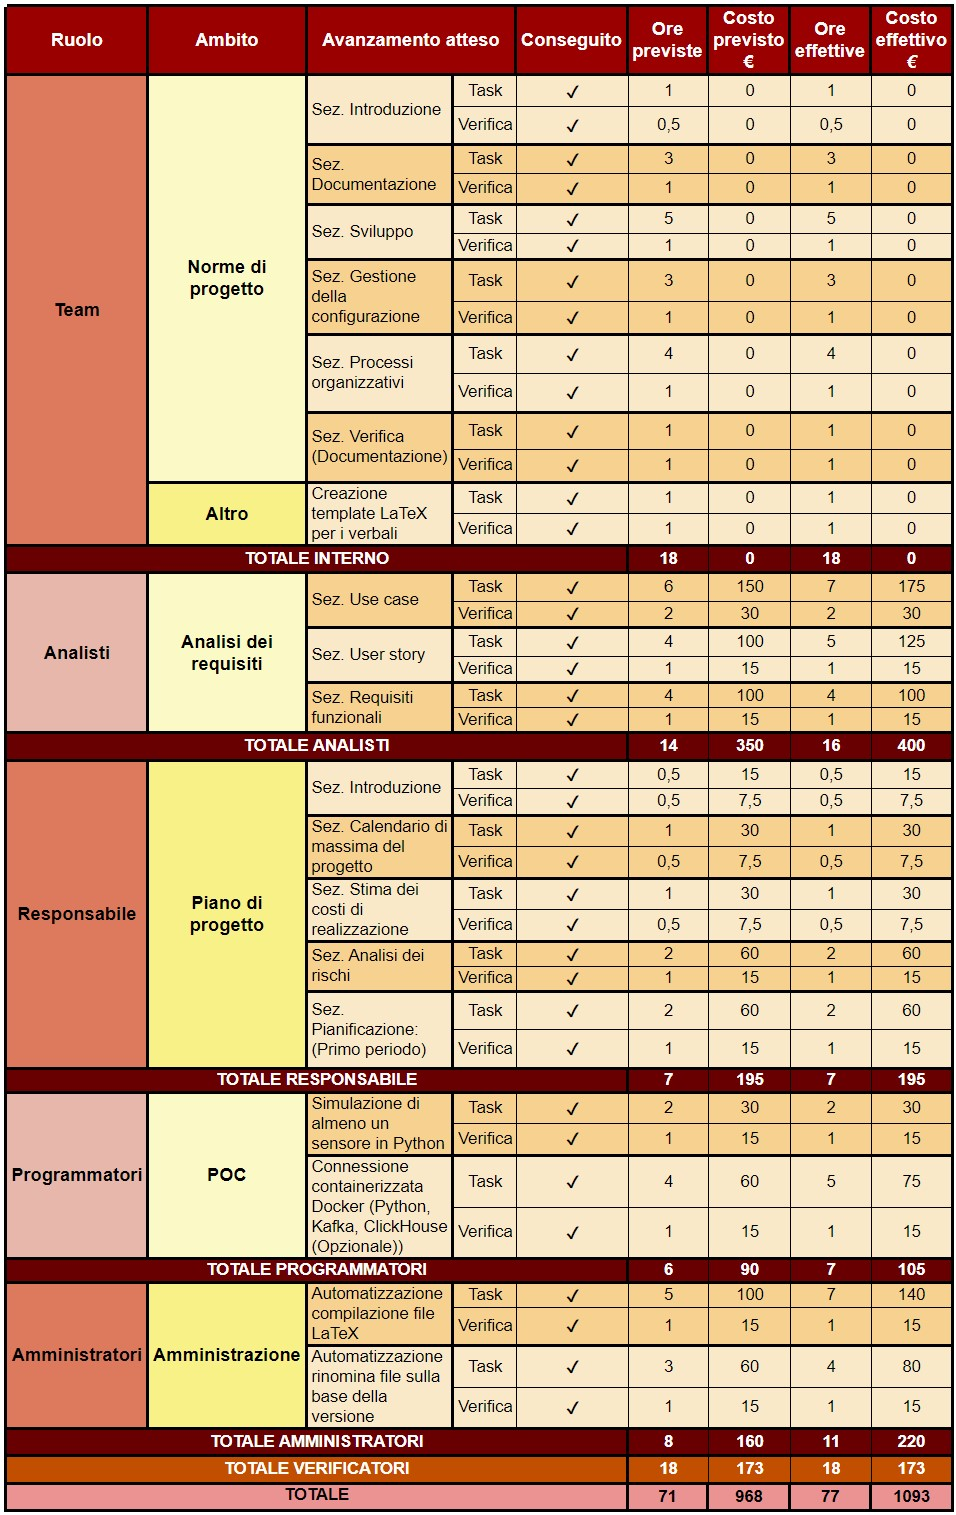
\includegraphics[height=1.0\textwidth]{../Images/periodo1.jpg}
    \caption{Primo periodo}
    \label{fig:1periodo}
\end{figure}

Al termine del primo periodo, l'ammontare parziale totale del costo del progetto è \textbf{ 1093\euro\ } e sono state completate il \textbf{100\%} delle attività attese.

\begin{figure}[ht]
    \centering
    \begin{minipage}[b]{0.45\textwidth}
        \centering
        \begin{tikzpicture}
            \pie[
                text=legend,
                color={blue!50, red!80}, 
                radius=2, 
                line width=0pt
            ]{8/Speso, 92/Rimanente}
        \end{tikzpicture}
        \caption{Grafico a torta del budget speso e rimanente preventivato nel primo periodo}
        \label{fig:GraficoTorta}
    \end{minipage}
    
    \vspace{1cm}

    \begin{minipage}[b]{0.70\textwidth}
        \centering
        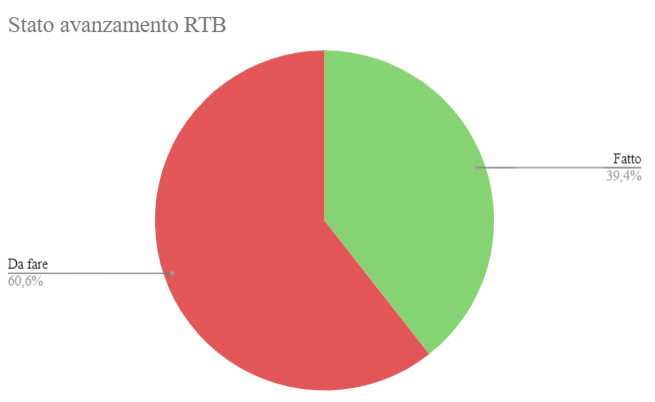
\includegraphics[width=0.7\textwidth]{../Images/avanzamento1Periodo.png}
        \caption{Avanzamento dei lavori RTB - primo periodo}
        \label{fig:AvRtb1}
    \end{minipage}
\end{figure}

\subsubsection*{Preventivo e consuntivo orario per membro}
Nel corso del primo periodo, sono state impiegate ore per l'esecuzione di attività interne, come dettagliato nella tabella precedente. Tali ore non sono state incluse nei costi e per svolgerle sono intervenuti i ruoli di responsabile e amministratore.
Per le attività registrate nei costi, sono stati assegnati i seguenti ruoli:

\begin{itemize}
    \item \textbf{Responsabile (Re):}
          \begin{itemize}
              \item F. Pozza.
          \end{itemize}
    \item \textbf{Amministratore (Am):}
          \begin{itemize}
              \item L. Skenderi.
          \end{itemize}
    \item \textbf{Analisti (An):}
          \begin{itemize}
              \item A. Barutta;
              \item R. Smanio.
          \end{itemize}
    \item \textbf{Verificatore (Ve):}
          \begin{itemize}
              \item E. Hysa.
          \end{itemize}
    \item \textbf{Programmatori (Pr):}
          \begin{itemize}
              \item N. Preto;
              \item D. Diotto.
          \end{itemize}
    \item \textbf{Progettista (Pt):}
          \begin{itemize}
              \item Nessuno.
          \end{itemize}
\end{itemize}

\paragraph{Preventivo orario} \hspace{1pt}

\begin{figure}[ht]
    \centering
    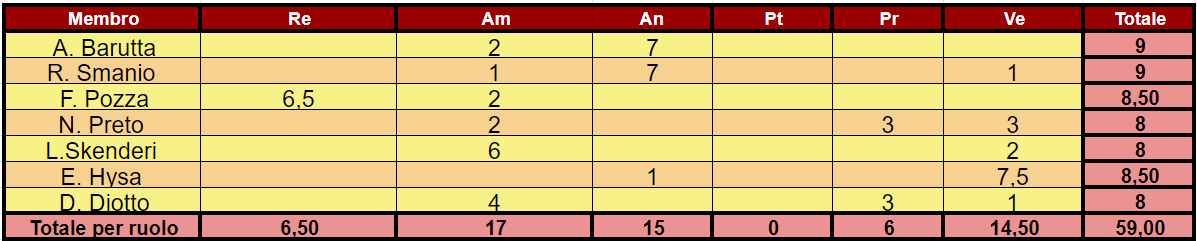
\includegraphics[width=0.9\textwidth]{../Images/preventivoOrario1Periodo.png}
    \caption{Preventivo orario per membro - primo periodo}
    \label{fig:Pv1}
\end{figure}

\begin{figure}[H]
    \centering
    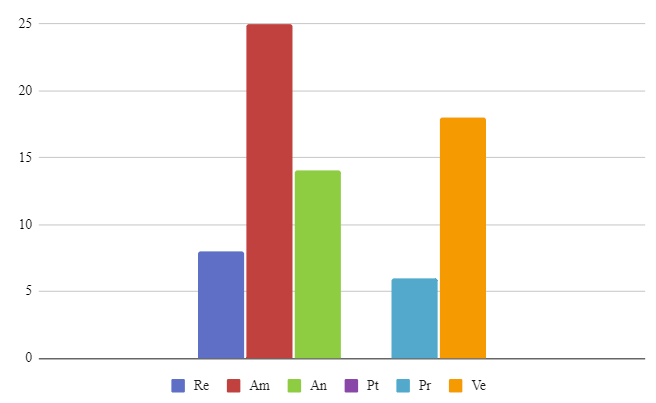
\includegraphics[width=0.6\textwidth]{../Images/preventivoDivisioneRuoli1Periodo.png}
    \caption{Istogramma preventivo della ripartizione oraria dei ruoli - primo periodo}
    \label{fig:PvD1}
\end{figure}

\paragraph{Consuntivo orario } \hspace{1pt}

\begin{figure}[ht]
    \centering
    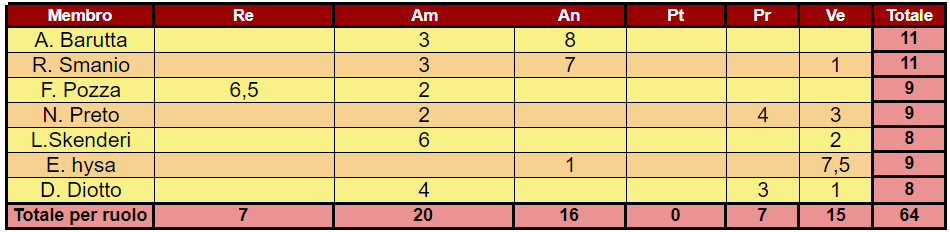
\includegraphics[width=0.9\textwidth]{../Images/consuntivoOrario1Periodo.png}
    \caption{Consuntivo orario per membro - primo periodo}
    \label{fig:Cv1}
\end{figure}

\begin{figure}[H]
    \centering
    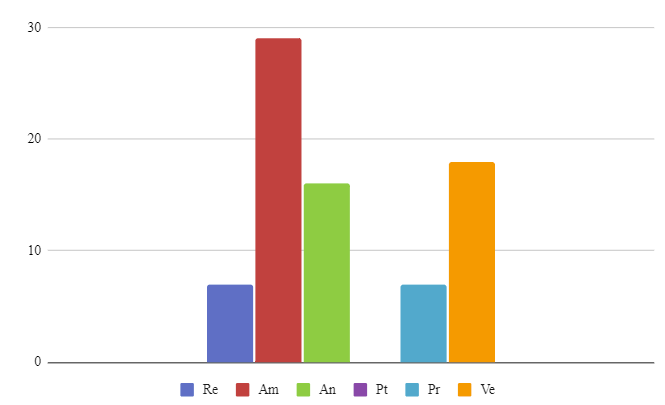
\includegraphics[width=0.6\textwidth]{../Images/consuntivoDivisioneRuoli1Periodo.png}
    \caption{Istogramma consuntivo della ripartizione oraria dei ruoli - primo periodo}
    \label{fig:CD1}
\end{figure}
